\documentclass{article}

% if you need to pass options to natbib, use, e.g.:
%     \PassOptionsToPackage{numbers, compress}{natbib}
% before loading neurips_2018

% ready for submission
% \usepackage{neurips_2018}

% to compile a preprint version, e.g., for submission to arXiv, add add the
% [preprint] option:
%     \usepackage[preprint]{neurips_2018}

% to compile a camera-ready version, add the [final] option, e.g.:
\usepackage[final]{nips_2018}

% to avoid loading the natbib package, add option nonatbib:
%     \usepackage[nonatbib]{neurips_2018}

\usepackage[utf8]{inputenc} % allow utf-8 input
\usepackage[T1]{fontenc}    % use 8-bit T1 fonts
\usepackage{hyperref}       % hyperlinks
\usepackage{url}            % simple URL typesetting
\usepackage{booktabs}       % professional-quality tables
\usepackage{amsfonts}       % blackboard math symbols
\usepackage{nicefrac}       % compact symbols for 1/2, etc.
\usepackage{microtype}      % microtypography
\usepackage{graphicx} 
\usepackage{float}

\title{Transfer Learning for Dog Breed Identification}

% The \author macro works with any number of authors. There are two commands
% used to separate the names and addresses of multiple authors: \And and \AND.
%
% Using \And between authors leaves it to LaTeX to determine where to break the
% lines. Using \AND forces a line break at that point. So, if LaTeX puts 3 of 4
% authors names on the first line, and the last on the second line, try using
% \AND instead of \And before the third author name.

\author{%
  Yizhou Chen\\
  \texttt{yic244@ucsd.edu} \\
  \And
  Zhongke Ma\\
  \texttt{z2ma@ucsd.edu} \\
  \And
  Qichao Zheng\\
  \texttt{q5zheng@ucsd.edu} \\
  \And
  Yisheng Ji\\
  \texttt{y3ji244@ucsd.edu} \\
}

\begin{document}
% \nipsfinalcopy is no longer used

\maketitle

\begin{abstract}
  In this project, we achieve classification of dog breeds from Stanford Dog Dataset which contains images of 120 dog breeds. ResNet50, DenseNet, VGG19 and InceptionV3 were used to extract the features. To get a better accuracy, we apply transfer learning on different networks such as VGG19 and InceptionV3. These networks were already built on Keras, which is a deep learning library and provides some popular neural networks. The result of this project can be used in identification of dogs in images.
\end{abstract}

\section{Introduction}

\subsection{Motivation}

Dog have become more and more important in our daily life, they appear as pets, transportation, drug detector and so on. Since different breed of dogs can help people in different way, the identification on breed of dogs have become commonly mentioned nowadays in many fields. Thus, we need a more accurate and efficiency way to classify the breed of dogs.

\subsection{Convolutional Neural Network}

Deep learning models have achieved remarkable results in computer vision in recent years. [1] As one of the deep learning networks, Convolutional Neural Network has widely used around the world for image classification. The CNN consist of neurons and the weights and biases of the neurons can be trained. Each neuron receives some inputs, performs a dot product and optionally follows it with a non-linearity. Convolutional layer, pooling layer, and fully-connected layer are the three main types of layers of Convolutional Neural Network.

In order to improve the performance of the network, CNN model nowadays has become deeper. However, as CNN become deeper, the cost of time and computing resource also become larger. Thus, to save time and make our calculation more efficient, we will use a pre-trained model in our project. Pre-trained model is a model already trained for some other task, we can re-train them in order to fit our task.

\begin{figure}[H]
	\centering
	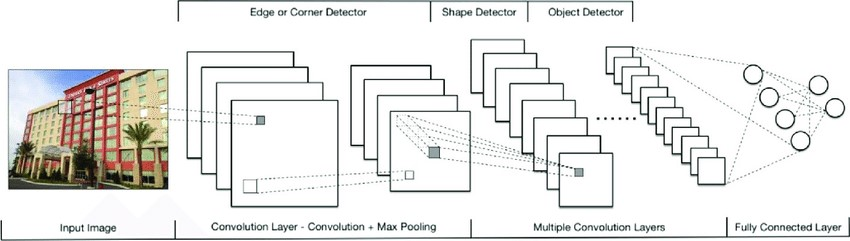
\includegraphics[width=3.5in]{pics/CNN} 
	\caption{Basic structure of CNN.}
\end{figure}

\section{Description of methods}

In our project, we apply several CNN models for image classification. ResNet-50, DenseNet, VGG19, InceptionV3 and transfer learning were used to build our neural networks.

%\subsection{ResNet-50}

%Deep convolutional neural networks have been widely used for image classification in order to get a better accuracy, however, as the neural networks become deeper, gradient vanishing and exploding problem will appear, which make the networks difficult to learn. ResNet are introduced to solve gradient vanishing and exploding problem and allow us to train much deeper networks. ResNet are a neural network consist of residual blocks, each residual block is 2 or 3 layers deep. By stacking residual blocks, ResNet can assure their performance when the networks become deeper. The main idea of ResNet is to add a shortcut connection from one layer to another much deeper layer. With Residual Networks, we can train deeper neural networks with more than 1000 layers. [2] ResNet-50 is a residual network with 50 layers, it uses bottleneck building block as its residual blocks. ResNet-50 can achieve 5.25\% top-5 error rate on the ImageNet validation set.

%\begin{figure}[H]
%	\centering
%	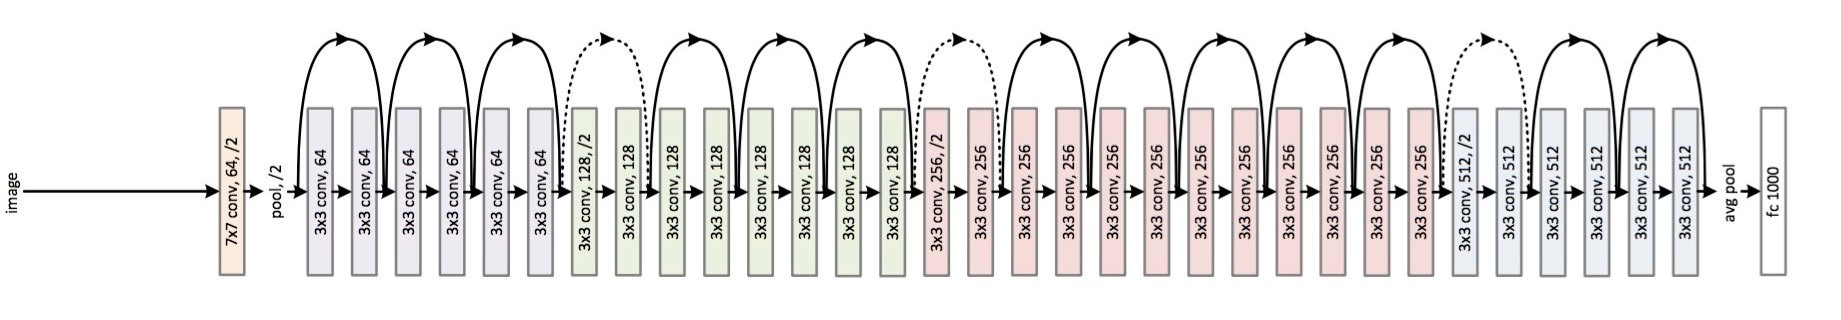
\includegraphics[width=3.5in]{pics/resnet} 
%	\caption{Basic architecture of ResNet.}
%\end{figure}

\subsection{DenseNet}

More and more models have shown that convolutional neural networks can become substantially deeper, more accurate, and efficient to train if they contain shorter connections between layers close to the input and those close to the output. Thus, Dense Convolutional Networks (DenseNet) was introduced. DenseNet consists of dense block, within each dense block, each layer is connected to every other layer in a feed-forward fashion. [3] In DenseNet, every layer is connected together by dense connectivity in order to have max information flow between the layers which means every layer have multiple inputs from other layers. 

In DenseNet, fewer parameters is needed, which means the parameters in DenseNet can be more efficiency than traditional neural networks. Besides, DenseNet can be deep while the layers can be slim. With all these advantages, DenseNet is easily to be trained.

\begin{figure}[H]
	\centering
	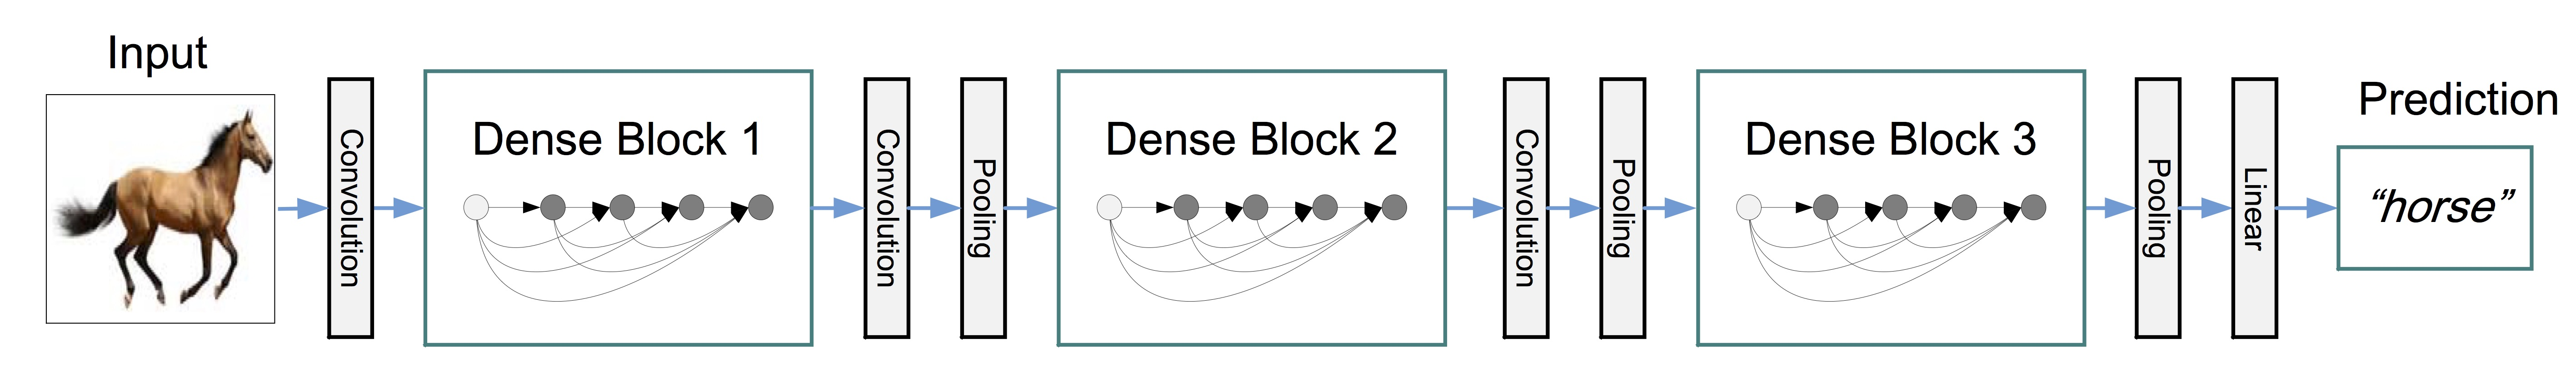
\includegraphics[width=3.5in]{pics/densenet} 
	\caption{A deep DenseNet with three dense blocks.}
\end{figure}

\subsection{VGG19}

VGG is a network of increasing depth using an architecture with very small convolution filters. With small convolution filters, the number of parameters can be reduced. The input of VGG is 224*224 RGB images. Then the input image will go through the convolutional layers, where filters with a small receptive field will be applied. Each convolutional layer has different depth, some of the convolutional layers will have a max-pooling layer followed, and the max-pooling layer has a 2$\times$2 pixels window with stride 2. With max-pooling layers, VGG can achieve spatial pooling. After the stack of convolutional layers three fully connected layers are followed. The first two layers have 4096 channels each, the third have 1000 channels. And the last layer of the network is a soft max layer. After the input go through the whole network, the output will be classification contains 1000 channels. VGG16 and VGG19 are the two most common models of VGG. VGG 16 has 16 weight layers which has about 138 million of parameters in total, while VGG19 has 19 weight layers which has about 144 million of parameters in total. [4] The model we will use in our project is VGG19, it can achieve 7.3\% top 5 error in ILSVRC.

\begin{figure}[H]
	\centering
	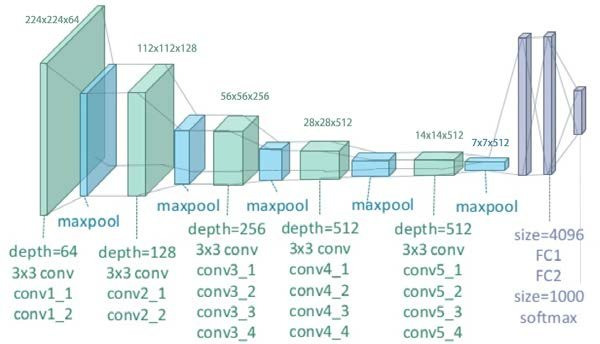
\includegraphics[width=3.5in]{pics/vgg} 
	\caption{VGG19 architecture.}
\end{figure}

\subsection{InceptionV3}

Inception is a deep convolutional neural network which provides a new state of the art for classification and detection. It makes a better use of the computing resources inside the network and makes the network deeper and wider while the computing budget is not affected. Inception networks consist of Inception modules. The main idea of the Inception architecture is to consider how an optimal local sparse structure of a convolutional vision network can be approximated and covered by readily available dense components. [5] To find the optimal local sparse structure, we assume that each unit of the previous layer refers to some part of the input image, which can find the clusters that focused on some particular region, thus, these clusters can be summed up by a 1*1 convolution in the following layer. And to avoid patch-alignment problem, the filter size of Inception has only 3 options: 1$\times$1, 3$\times$3 and 5$\times$5. To keep the computing complexity stable, Inception network uses dimensionality reduction which can reduce the feature maps from 192 to 16.

InceptionV3, as the improved model of Inception networks, has 42 layers, which is much deeper than GoogLeNet, the first model of Inception networks. The improvement InceptionV3 make is that they applied factorization of convolutions and improved normalization in the networks. [6] Comparing with GoogLeNet, the top 5 error of InceptionV3 is improved from 6.67\% to 4.49\%.


\begin{figure}[H]
	\centering
	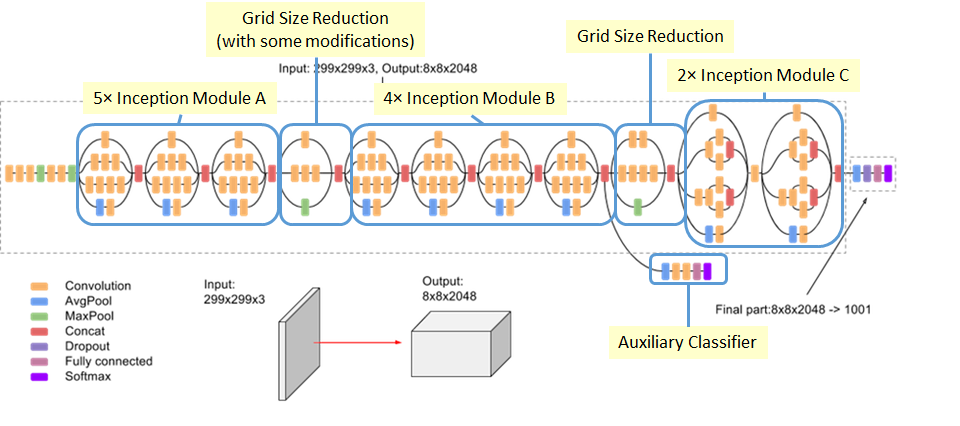
\includegraphics[width=3.5in]{pics/inception} 
	\caption{InceptionV3 architecture.}
\end{figure}

\subsection{Transfer learning}

Transfer learning is a machine learning technique where a model trained on one task is re-purposed on a second related task. In traditional CNN for image classification, usually the earlier layers are to detect edges, while deeper layers will try to detect some specific features. With transfer learning, we can use the earlier layers to re-train the deeper layers. The main benefit transfer learning is saving training time without hurting the performance. Also, with transfer learning, we can use less data to train the neural networks. 

\section{Implementation Details}

In this section, we 

\newpage
\section{Experimental Settings}

\subsection{Datasets}

The dataset we used in this project is Stanford Dogs Dataset, which contains images of 120 breeds of dogs from around the world, such as Chihuahua, Japanese spaniel and Rhodesian ridgeback. This dataset has been built using images and annotation from ImageNet for the task of fine-grained image categorization. There are totally 20580 images in this dataset, 12000 images in the training set and 8580 in the testing set.

\begin{figure}[H]
	\centering
	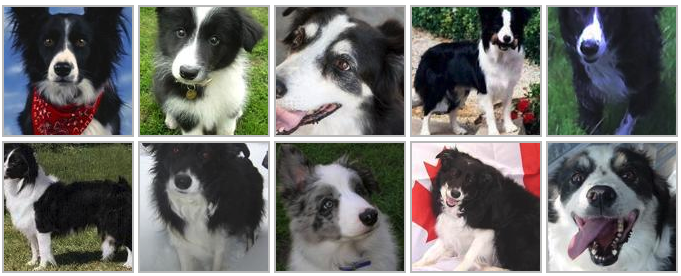
\includegraphics[width=3.5in]{pics/dogs} 
	\caption{Stanford Dogs Dataset.}
\end{figure}


\subsection{Training Parameters}
\subsection{Hardware Used}

\newpage
\section{Results}

\subsection{InceptionV3}
\subsection{DenseNet121}
\subsection{VGG19}
\begin{table}[h]
	\centering
	
	\begin{tabular}{|c|c|}
		\hline
		Number of selected categories & Accuracy \\\hline
		20 & 87.31\\
		40 & 83.53\\
		60 & 80.01\\
		80 & 76.29\\
		100 & 74.42\\
		120 & 70.67\\
		\hline
	\end{tabular}
\caption{Accuracy versus categories selected}
\end{table}
\begin{figure}[H]
	\centering
	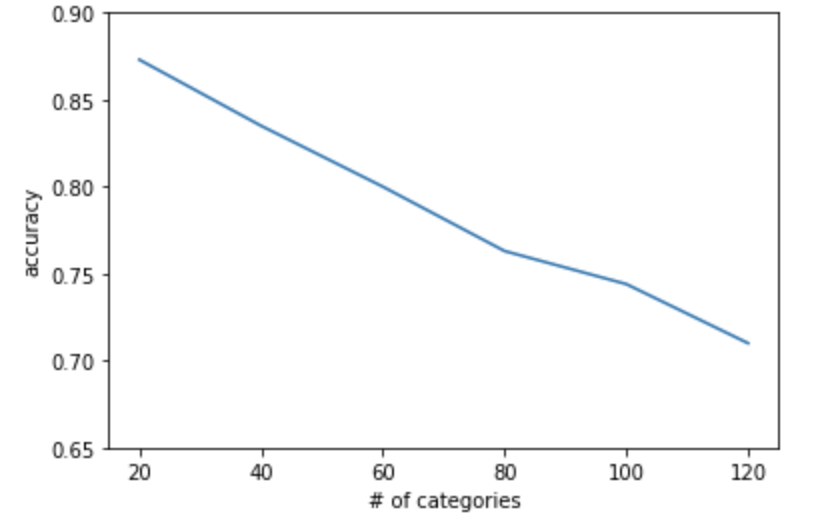
\includegraphics[width=3.5in]{pics/vgg19_1} 
	\caption{Accuracy versus categories selected}
\end{figure}
The test accuracy of our algorithm is 70.07\% if all 120 dog breeds are included. 
\subsection{Comparision}

\newpage
\section{Discussion}
\begin{figure}[H]
	\centering
	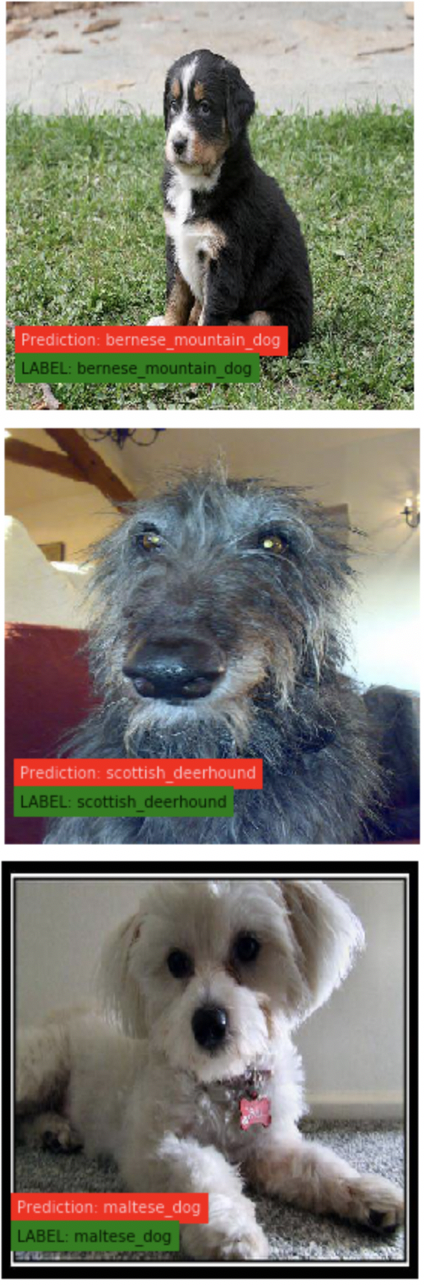
\includegraphics[width=1.5in]{pics/correct_samples} 
	\caption{Some correctly classified samples}
\end{figure}
\begin{figure}[H]
	\centering
	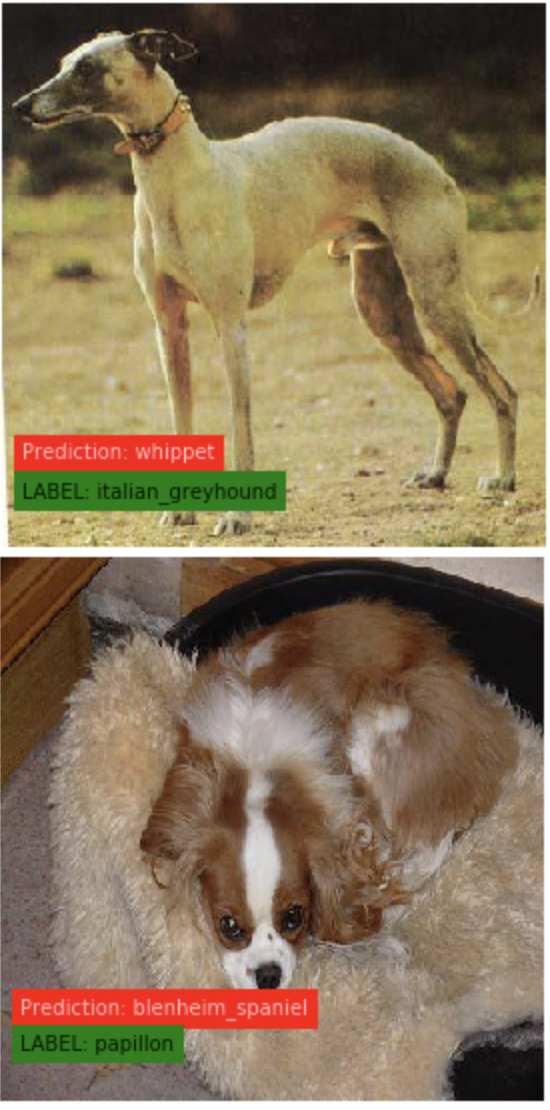
\includegraphics[width=1.5in]{pics/wrong_samples} 
	\caption{Some misclassified samples}
	
\end{figure}
From the above misclassified samples, the color of the background is so much close to the dog, which will  We also notice that in the training test there exist some images contains more than one dog and same image appears twice in two different breeds as shown in below. This type of error seems not solvable via programming. 
\begin{figure}[H]
	\centering
	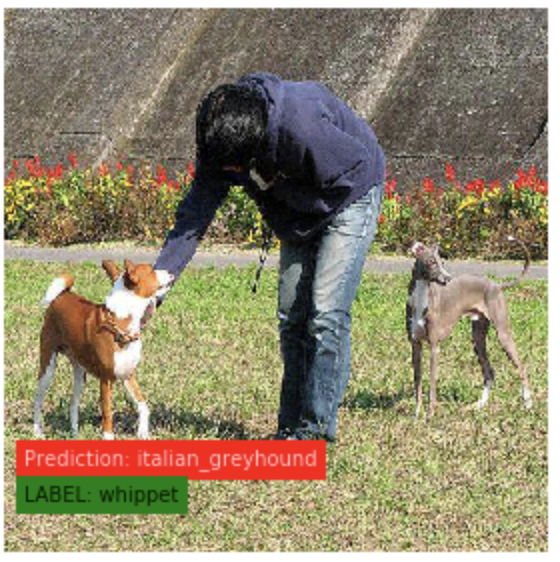
\includegraphics[width=2in]{pics/two_dogs} 
	\caption{Sample of more than one dogs}
\end{figure}


\section{Appendix}


\section*{References}

\medskip

\small

[1] Kim Y. Convolutional neural networks for sentence classification[J]. arXiv preprint arXiv:1408.5882, 2014.

[2] He K, Zhang X, Ren S, et al. Deep residual learning for image recognition[C]//Proceedings of the IEEE conference on computer vision and pattern recognition. 2016: 770-778.

[3] Huang G, Liu Z, Van Der Maaten L, et al. Densely connected convolutional networks[C]//CVPR. 2017, 1(2): 3.

[4] Simonyan K, Zisserman A. Very deep convolutional networks for large-scale image recognition[J]. arXiv preprint arXiv:1409.1556, 2014.

[5] Szegedy C, Liu W, Jia Y, et al. Going deeper with convolutions[C]//Proceedings of the IEEE conference on computer vision and pattern recognition. 2015: 1-9.

[6] Szegedy C, Vanhoucke V, Ioffe S, et al. Rethinking the inception architecture for computer vision[C]//Proceedings of the IEEE conference on computer vision and pattern recognition. 2016: 2818-2826.


\end{document}
